\documentclass[tikz,border=2mm]{standalone}
\usepackage[T1]{fontenc}
\usepackage[utf8]{inputenc}
\usepackage[scaled]{helvet}
\renewcommand{\familydefault}{\sfdefault}
\usetikzlibrary{arrows.meta,positioning,calc}
\definecolor{dunkel}{HTML}{1F3A5F}
\definecolor{mittel}{HTML}{5B7FA6}
\definecolor{hell}{HTML}{DCE6F0}
\definecolor{text}{HTML}{222222}
\tikzset{
  every node/.style={text=text},
  pfeil/.style={line width=2pt,draw=dunkel,-{Triangle[length=3.5mm,width=4mm]}},
  doppelpfeil/.style={line width=4pt,draw=dunkel,{Triangle[length=4mm,width=7mm]}-{Triangle[length=4mm,width=7mm]}},
  duennpfeil/.style={line width=1pt,draw=mittel,{Stealth[length=2.5mm]}-{Stealth[length=2.5mm]}},
}

\begin{document}
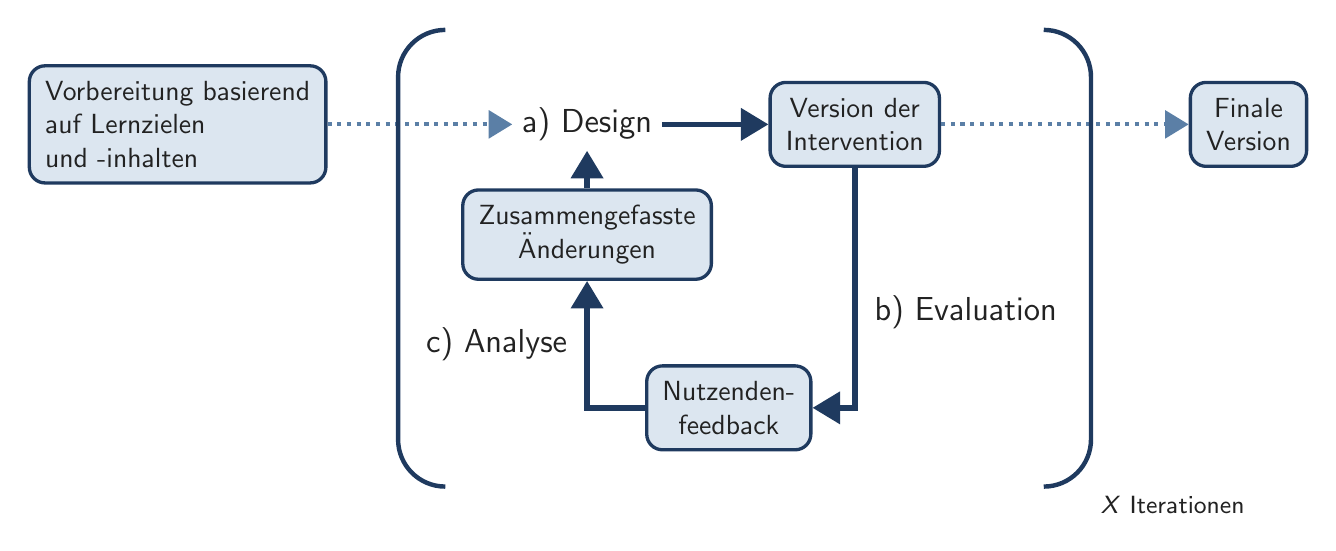
\begin{tikzpicture}[
    box/.style={draw=dunkel,line width=1.2pt,rounded corners=2mm,fill=hell,align=center,inner sep=2mm},
    phase/.style={font=\large},
    gepunktet/.style={line width=1.5pt,draw=mittel,dotted,-{Triangle[length=3mm,width=3.5mm]}},
    klammer/.style={line width=1.6pt,draw=dunkel},
  ]
  \node[box,align=left] (prep) at (0,3) {Vorbereitung basierend\\auf Lernzielen\\und -inhalten};
  \node[phase] (design) at (5.2,3) {a) Design};
  \node[box] (version) at (8.6,3) {Version der\\Intervention};
  \node[box] (final) at (13.6,3) {Finale\\Version};
  \node[box] (changes) at (5.2,1.6) {Zusammengefasste\\Änderungen};
  \node[box] (feedback) at (7.0,-0.6) {Nutzenden-\\feedback};

  \draw[gepunktet] (prep.east) -- (design.west);
  \draw[pfeil] (design.east) -- (version.west);
  \draw[gepunktet] (version.east) -- (final.west);
  \draw[pfeil] (version.south) |- node[pos=0.3,right,phase,xshift=1mm] {b) Evaluation} (feedback.east);
  \draw[pfeil] (feedback.west) -| node[pos=0.75,left,phase,xshift=-1mm] {c) Analyse} (changes.south);
  \draw[pfeil] (changes.north) -- (design.south);

  \draw[klammer] (3.4,4.2) to[out=180,in=90] (2.8,3.6) -- (2.8,-1.0) to[out=-90,in=180] (3.4,-1.6);
  \draw[klammer] (11.0,4.2) to[out=0,in=90] (11.6,3.6) -- (11.6,-1.0) to[out=-90,in=0] (11.0,-1.6);
  \node[anchor=north west,font=\small] at (11.6,-1.6) {\textit{X} Iterationen};
\end{tikzpicture}
\end{document}
